\begin{figure}[h]
    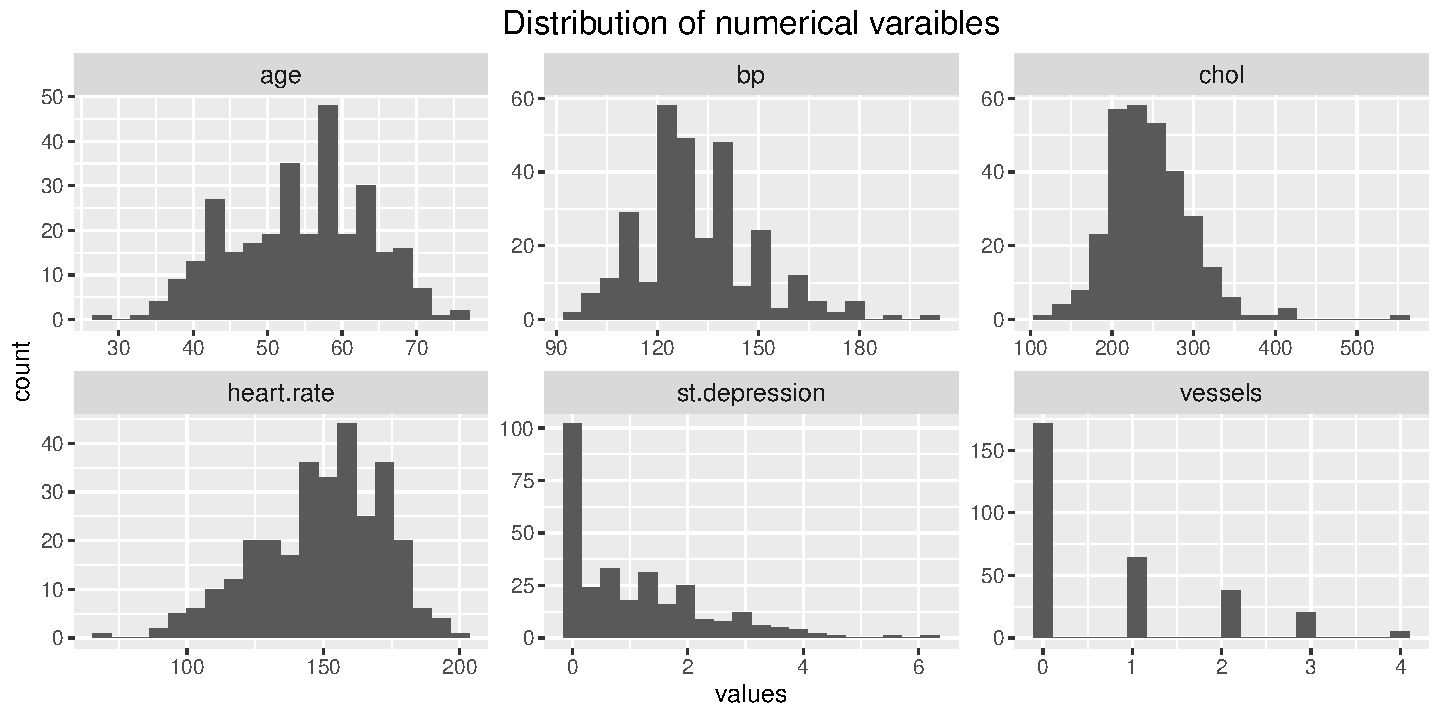
\includegraphics[width=\linewidth]{23.numerical.distribution.pdf}
    \caption{\centering Histogram of numerical features}
\end{figure}

There are 6 numerical variables in the dataset, 5 of which are different types of clinical metrics 
(\texttt{bp}, \texttt{chol}, \texttt{heart.rate}, \texttt{st.depression}, \texttt{vessels}). In general, by plotting the histograms for the variables, it is observed that some of the features (\texttt{bp}, \texttt{heart.rate}, \texttt{chol}) are 'close' to a normal distribution, whilst others are heavily \textit{left-skewed} (\texttt{age}) or \textit{right-skewed} (\texttt{st.depression}, \texttt{vessels}).


The relationship of number variables and the response is tested on a faceted box-plot. By visually comparing the distribution mean of each group, it can be seen that there are 

\begin{itemize}
    \item \textbf{Strong correlation} between varibles \texttt{age}, \texttt{heart.rate}, \texttt{vessels}, \texttt{st.depression} and the response variable;
    \item \textbf{Weak correlation} between \texttt{bp} and \texttt{chol} and the response variable
\end{itemize}

\begin{figure}[h]
    \centering
    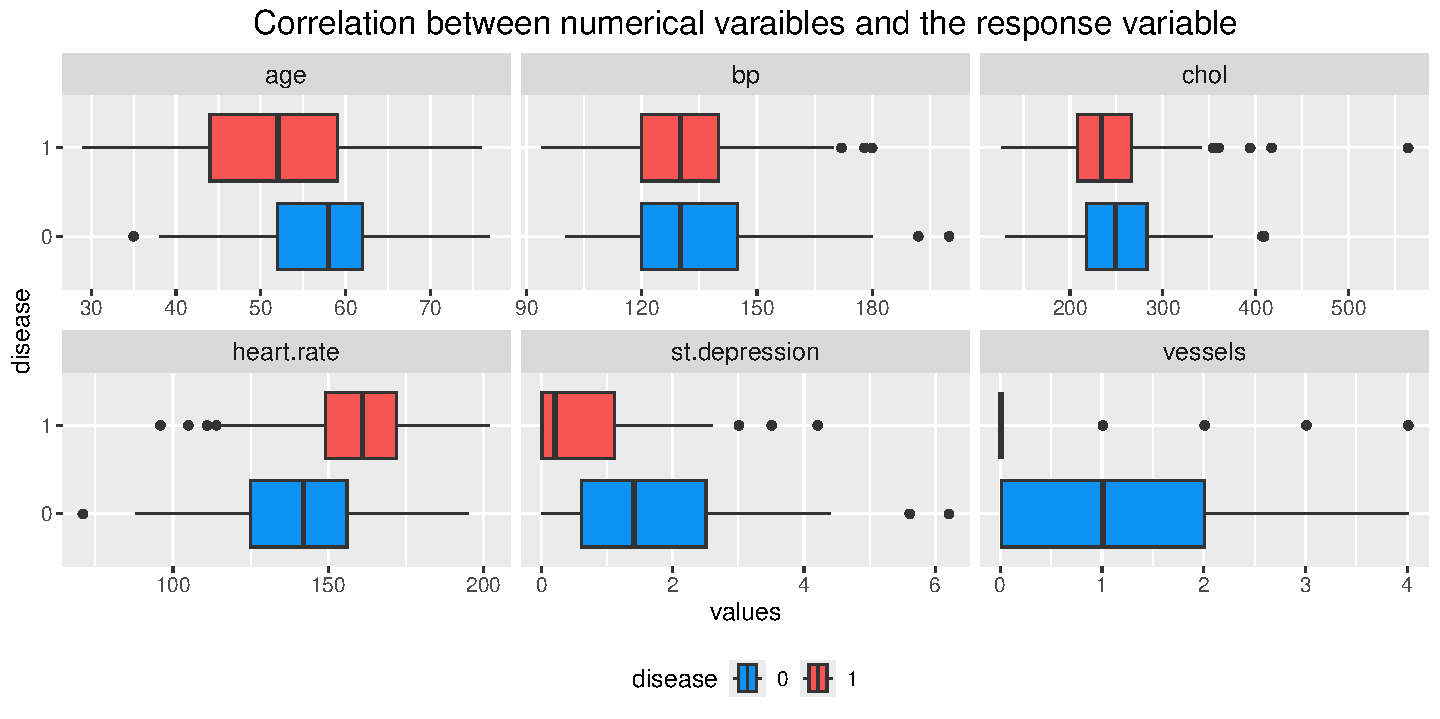
\includegraphics[width=\linewidth]{23.numerical.correlation.to.response.pdf}
    \caption{\centering Boxplot correlation with disease}
\end{figure}

To test for normality for each variables, a QQ-plot is used for visualisation, along with the p-value from the \textit{Shapiro-Wilk normality test} \citep{shapirotest}. As no variables are normally distributed (all \( p < 10^{-2} \)), normality transformations are also considered. In this case, the transformation of interest is the \textit{Box-Cox transformation}, a parametric transformation that generalises power and logarithmic transformations on positive variables with a single parameter \( \lambda \):

\[
    B_\lambda(x) = \begin{cases}
        \frac{x^\lambda - 1}{\lambda}   & \text{if \( \lambda \ne 0 \)} \\
        \ln{x}                          & \text{if \( \lambda  =  0 \)}
    \end{cases}
\]

For non-negative variables, a \( x \mapsto x + \varepsilon \) transformation, where \( \varepsilon = 0.01\), is applied before Box-Cox to prevent the transformation being undefined at \( x = 0 \).

Different values of \( \lambda \) in the range \( [-5, 5] \) are tested, the value of which yields the best \textit{Shapiro-Wilk's p-value} is retained. It can be observed that \texttt{age}, \texttt{bp}, \texttt{chol} and \texttt{heart.rate} are Box-Cox transformable to a normally distributed variable, within a \( 99\% \) level of significance. In contrast, heavy right-skewed variables (\texttt{st.depression} and \texttt{vessels}) fail to be normally transformable by the Box-Cox transformation.

\begin{figure}[h]
    \centering
    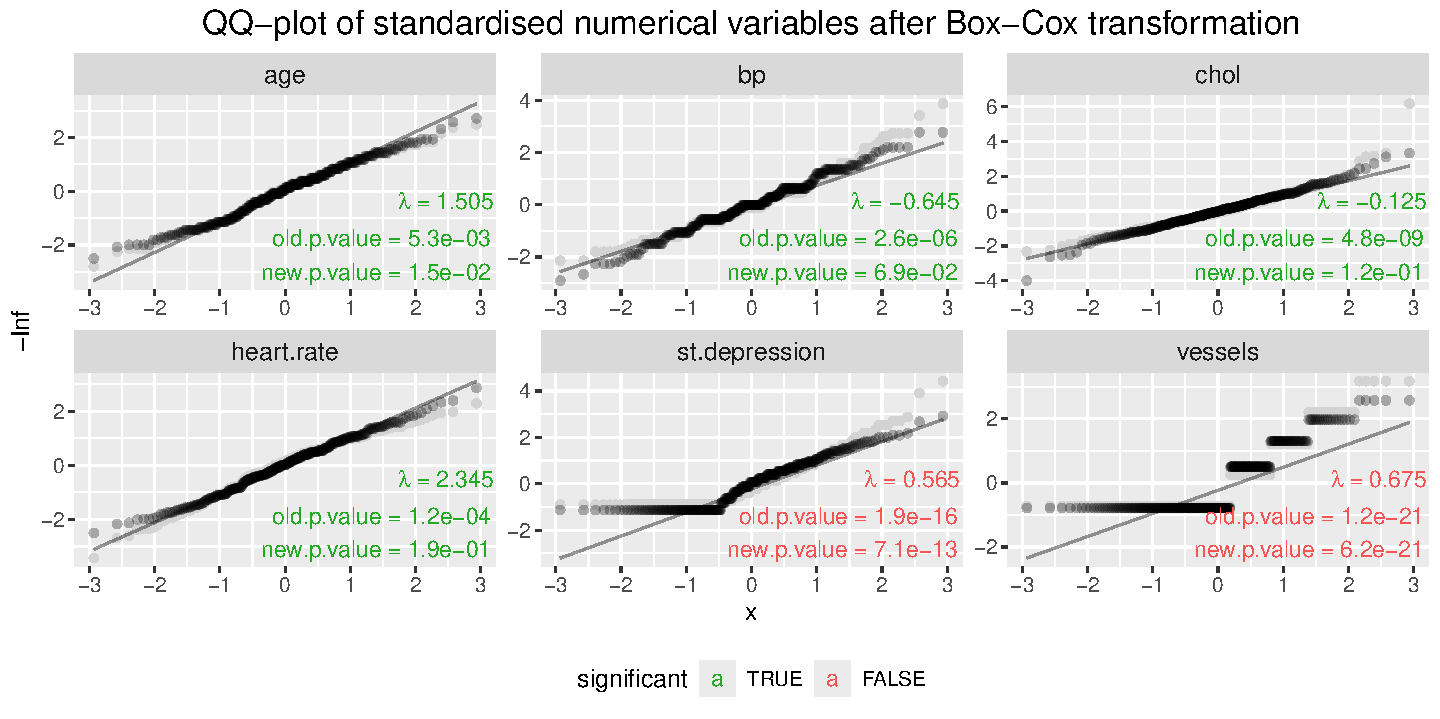
\includegraphics[width=\linewidth]{23.numerical.boxcox.qq.pdf}
    \caption{\centering Best Box-Cox transformation for each numerical variable}
\end{figure}

